% FastLane progress report -- ACL-style layout, single column.
% Build: cd report && pdflatex fastlane_report && bibtex fastlane_report && pdflatex fastlane_report && pdflatex fastlane_report
\documentclass[11pt,a4paper]{article}

\usepackage[T1]{fontenc}
\usepackage[utf8]{inputenc}
\usepackage{times}
\renewcommand{\ttdefault}{lmtt}
\usepackage{microtype}
\usepackage[a4paper,top=2.5cm,bottom=2.5cm,left=2.5cm,right=2.5cm]{geometry}
\usepackage{graphicx}
\usepackage{booktabs}
\usepackage{tabularx}
\usepackage{array}
\usepackage{amsmath}
\usepackage{xcolor}
\usepackage{url}
\usepackage[small,labelfont=bf]{caption}
\usepackage{tikz}
\usetikzlibrary{positioning,arrows.meta,fit}
\PassOptionsToPackage{hyphens}{url}
\usepackage[hidelinks]{hyperref}
\newcommand{\hcell}[1]{\begin{tabular}[b]{@{}r@{}}#1\end{tabular}}  % right-aligned two-line table header

% ACL-like headings: section \large bold, subsection \normalsize bold, paragraph run-in bold.
\makeatletter
\renewcommand\section{\@startsection{section}{1}{\z@}{-2.2ex plus -0.5ex minus -0.2ex}{1.1ex plus 0.2ex}{\large\bfseries\raggedright}}
\renewcommand\subsection{\@startsection{subsection}{2}{\z@}{-1.8ex plus -0.5ex minus -0.2ex}{0.8ex plus 0.2ex}{\normalsize\bfseries\raggedright}}
\renewcommand\paragraph{\@startsection{paragraph}{4}{\z@}{1.2ex plus 0.5ex minus 0.2ex}{-1em}{\normalsize\bfseries}}
\makeatother
\setlength{\parindent}{1em}
\setlength{\emergencystretch}{2em}
\setlength{\parskip}{0pt}
% Let several floats share a text page so tables stay near their text instead of piling up at the end.
\renewcommand{\topfraction}{0.85}\renewcommand{\bottomfraction}{0.6}\renewcommand{\textfraction}{0.1}
\renewcommand{\floatpagefraction}{0.75}\setcounter{topnumber}{3}\setcounter{bottomnumber}{2}\setcounter{totalnumber}{5}
\makeatletter\setlength{\@fptop}{0pt}\setlength{\@fpsep}{10pt plus 2pt}\makeatother  % float pages start at the top
\setlength{\textfloatsep}{10pt plus 2pt minus 2pt}
\setlength{\floatsep}{8pt plus 2pt minus 2pt}
\setlength{\intextsep}{8pt plus 2pt minus 2pt}
\renewcommand{\arraystretch}{1.1}
\newcolumntype{L}{>{\raggedright\arraybackslash}X}
\newcommand{\cmd}[1]{{\small\ttfamily\def\_{\textunderscore\allowbreak}#1}}  % code names may break after "_"
\newcommand{\Rs}{Rs~}
\let\olditemize\itemize
\renewcommand{\itemize}{\olditemize\setlength{\itemsep}{1pt}\setlength{\parskip}{0pt}\setlength{\topsep}{2pt}}

\title{\Large\bfseries FastLane: A Voice Agent That Uses a Small Model for Easy Turns\\
and a Large Model Only for Hard Ones\\[4pt]
\normalsize\normalfont LMA Group Project 2026 --- Mid-Submission Report (30 October 2026)}
\author{
  \textbf{Team: Chaturvedi and Sons}\\[4pt]
  \begin{tabular}{c@{\hspace{3em}}c@{\hspace{3em}}c}
  \textbf{Noel Alex Jacob} & \textbf{Aviral Tyagi} & \textbf{Sankalp Chaturvedi}\\
  2025201085 & 2025201086 & 2025201083\\[4pt]
  \multicolumn{3}{c}{\textbf{KSPSVLN Siddardha Kumar Kavuri}}\\
  \multicolumn{3}{c}{2025201061}
  \end{tabular}\\[6pt]
  {\small GitHub: \url{https://github.com/Sankalp0109/FastLane-Adaptive-Voice-Agent}}
}
\date{}

\begin{document}
\maketitle
\vspace{-1.2em}

\begin{abstract}
\noindent FastLane is a phone agent that books, changes and cancels movie tickets, bus tickets and restaurant tables for
Indian-English callers. A LoRA-tuned Qwen2.5-3B answers every turn first and passes only hard turns to a large API
model (gpt-oss-120b) or to staff; every action goes through a tool and policy gateway that enforces booking rules
and a read-back confirmation in code. This report describes everything built so far: a deterministic practice
booking system with 11 tools, a 360-call test set with a simulated caller, a data generator that runs an oracle agent
through the real orchestrator, five data versions and five Kaggle training sessions, and a local voice pipeline (Silero
VAD, Whisper, Kokoro). Offline, the tuned small model routes 99.3\% of held-out steps correctly (untuned: 89.1\%) and
fills tool arguments exactly in 99.0\% (untuned: 26.8\%). On 24 end-to-end calls, FastLane with the fixes found in
the pilots succeeds in 95.8\% of calls (untuned small model: 79.2\%; untuned small model alone, B2: 29.2\%) with the
lowest median model time per turn (1.55\,s). The ablations support two hypotheses: without date and alternative tools
(A2) the large model is called about twice as often, and with rules only in the prompt (A3) 15 of 24 calls make a
booking change the caller never confirmed, against none for FastLane. The large-model-only baseline (B1) could not be
run before this report because the free API quota ran out. On real Indian-English speech
(Svarah), Sarvam's recogniser has the lowest error (5.8\% WER vs.\ 9.5--10.5\% for Whisper), and a TTS$\rightarrow$STT
round trip shows that recogniser noise roughly triples the tuned model's argument errors (98.1\% $\rightarrow$ 94.3\%
exact). We report each iteration with the reason it was needed, and what remains for the final comparison.
\end{abstract}

% =====================================================================================================================
\section{Introduction}

A voice agent has about a second to reply before callers talk over it or repeat themselves. Most agents send every
turn to a large API model, which adds 1--3\,s per turn and costs too much for a small cinema, bus operator or
restaurant. Yet most turns in a booking call are easy (a date, a seat count, a name, a ``yes'' to a read-back); only
a few are hard (``next Friday'', a sold-out show, a caller changing their mind, a request that breaks a rule). A wrong
booking is worse than a slow one, and recognisers often mishear Indian names, places and numbers. Our question is
\emph{for each turn, which model should reply}, judged on speed, correctness and safety together.

The proposal states three research questions: (RQ1) can a LoRA-tuned small model that both answers easy turns and
decides when to pass a turn on cut time per turn by $\geq$50\% without a real drop in booking success compared with a
large-model-only agent; (RQ2) does moving rules and routine work (dates, alternatives, policy checks) from the prompt
into code reduce large-model calls and unsafe bookings; (RQ3) does a small model trained only on movies and buses
still work on restaurants. They come with seven hypotheses (Table~\ref{tab:hyp}).

\paragraph{Progress and structure of this report.} Table~\ref{tab:progress} summarises progress by phase of the
plan: Phases 0--7 are done, and Phase 8 (the full comparison) has started with baseline and ablation runs on a
24-call sample. The report follows the mid-submission items: the system (Section~\ref{sec:system}), datasets
(Section~\ref{sec:data}), baselines, ablations and metrics (Section~\ref{sec:eval}), training
(Section~\ref{sec:training}), results of all experiments run so far (Section~\ref{sec:results}), challenges and
mitigation (Section~\ref{sec:lessons}), the status of each hypothesis (Section~\ref{sec:status}) and the remaining
work with a timeline to the final submission on 15 November (Section~\ref{sec:todo}). All code is in one Python
package (about 10.4k lines in \cmd{src/fastlane}, 192 passing tests) on GitHub, with the Kaggle notebook, result
files and a run log recording every experiment.

\begin{table}[tbp]
\centering\small
\begin{tabularx}{\linewidth}{@{}>{\raggedright\arraybackslash}p{4.0cm}>{\raggedright\arraybackslash}p{2.3cm}L@{}}
\toprule
Phase & Status & What exists \\
\midrule
0 Scaffolding & done & Python package, CLI (\cmd{fastlane \dots}), 192 tests \\
1 Practice world & done & SQLite booking system for 3 domains, fixed seed, snapshot/restore per call \\
2 Gateway and booking record & done & 11 tools, rules in code, read-back gate, identity check, error injection, 2 rules added after pilots \\
3 Retrieval & done (corpus partial) & BM25 over 25 policy documents, old/new policy versions, early lookup; Recall@3 0.967 \\
4 Models and orchestrator & done & all 12 systems run end to end; large model with rate-limit backup \\
5 Evaluation harness & done & 360-call test set, LLM caller, resumable runner, all proposal metrics \\
6 Training & v1--v3 trained; v4/v5 data ready & 5 data versions, 5 Kaggle sessions; v3: route 99.3\%, arguments 99.0\% offline \\
7 Speech & done & browser voice demo, STT comparison on Svarah, TTS$\rightarrow$STT noise for training \\
8 Experiments & started & FastLane, B2, A2, A3, A8 on 24 calls (A1 from the pilot); B1, B3 blocked by API quota \\
\bottomrule
\end{tabularx}
\caption{Progress by phase of the project plan.}
\label{tab:progress}
\end{table}

% =====================================================================================================================
\section{Related Work}

Model routers such as FrugalGPT (a cascade of LLMs of increasing cost) and RouteLLM (a router trained on
preference data) choose one model per \emph{question} on single-turn benchmarks. FastLane routes \emph{per turn}
inside a long, tool-using dialogue, and the router is the small model itself, so easy turns pay no routing delay.
Tool-agent benchmarks such as $\tau$-bench check the final database state with a simulated user, which we adopt, but
do not measure latency, so they reward always using the largest model; we report speed, success and unsafe actions
together. We tune Qwen2.5-3B-Instruct with LoRA on a 4-bit base (QLoRA) and serve it with MLX; the speech layer uses
Silero VAD, Whisper, Sarvam's Indian-language recogniser and Kokoro TTS.

% =====================================================================================================================
\section{System}\label{sec:system}

\begin{figure}[tbp]
\centering
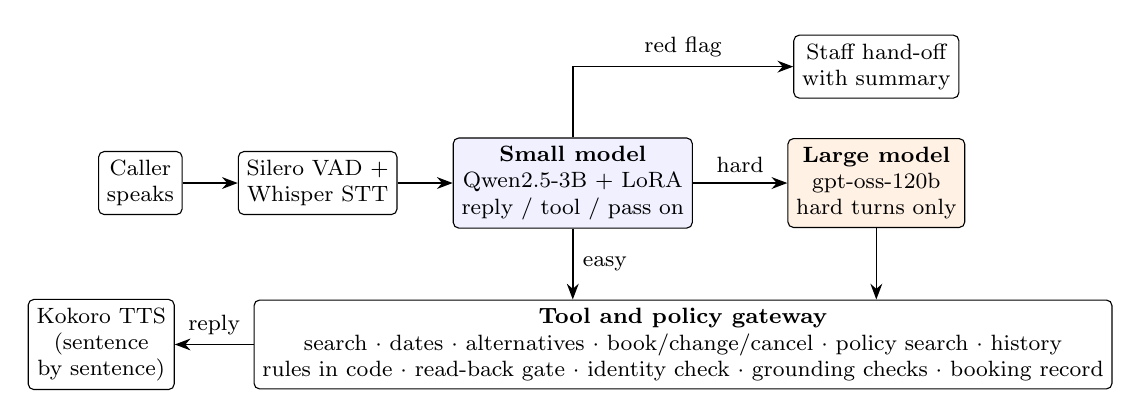
\begin{tikzpicture}[font=\footnotesize, node distance=6mm and 7mm,
  box/.style={draw, rounded corners=2pt, align=center, minimum height=8mm, inner sep=3pt, fill=white},
  arr/.style={-{Stealth[length=2mm]}, semithick}]
\node[box] (caller) {Caller\\speaks};
\node[box, right=of caller] (stt) {Silero VAD +\\Whisper STT};
\node[box, right=of stt, fill=blue!6] (small) {\textbf{Small model}\\Qwen2.5-3B + LoRA\\reply / tool / pass on};
\node[box, right=12mm of small, fill=orange!10] (large) {\textbf{Large model}\\gpt-oss-120b\\hard turns only};
\node[box, above=5mm of large] (staff) {Staff hand-off\\with summary};
\node[box, below=9mm of small, xshift=14mm] (gw) {\textbf{Tool and policy gateway}\\ search $\cdot$ dates $\cdot$ alternatives $\cdot$ book/change/cancel $\cdot$ policy search $\cdot$ history\\
rules in code $\cdot$ read-back gate $\cdot$ identity check $\cdot$ grounding checks $\cdot$ booking record};
\node[box, left=10mm of gw] (tts) {Kokoro TTS\\(sentence\\by sentence)};
\draw[arr] (caller) -- (stt);
\draw[arr] (stt) -- (small);
\draw[arr] (small) -- node[above]{hard} (large);
\draw[arr] (small.north) |- node[pos=0.75, above]{red flag} (staff.west);
\draw[arr] (small) -- node[right]{easy} (gw.north -| small);
\draw[arr] (large.south) -- (gw.north -| large);
\draw[arr] (gw) -- node[above]{reply} (tts);
\end{tikzpicture}
\caption{FastLane. Every caller turn goes to the tuned small model, which replies (optionally with a tool call),
passes the turn to the large model, or hands it to staff. Neither model writes to the booking system directly.}
\label{fig:arch}
\end{figure}

\paragraph{Practice world.} One SQLite database built from a fixed seed with a fixed ``now'' (Thursday 15 October
2026, so Dussehra and Diwali fall inside the booking window): 4 cinemas, 12 screens, 9 films and 1,440 shows with
seat maps (41,110 seats taken); 6 bus routes between Hyderabad and Bengaluru, Vijayawada and Chennai with 720 trips
(6,966 seats taken); 3 Tandoor Tales branches with 45 tables and 2,613 existing reservations; 200 callers with 510
past bookings (for returning callers) and 70 open bookings. Some shows, trips and slots are sold out on purpose for
the ``needs an alternative'' calls. Each test call starts from a snapshot of the same database.

\paragraph{Gateway and rules.} The gateway exposes eleven tools with validated arguments:
\cmd{search\_inventory}, \cmd{resolve\_date}, \cmd{find\_alternatives}, \cmd{create\_booking}, \cmd{modify\_booking},
\cmd{cancel\_booking}, \cmd{lookup\_booking}, \cmd{get\_caller\_history}, \cmd{search\_policy}, \cmd{send\_sms} and
\cmd{handoff\_to\_staff}. Rules are enforced in code, not in the prompt:
at most 10 movie tickets and changes up to 4\,h before the show; at most 6 bus seats, name/age/gender for every
passenger, refunds of 90/75/50/25\% by hours to departure; restaurant party limits (12/10/8 by branch) and a deposit
for large groups. A create, change or cancel first returns a read-back that must be spoken to the caller; the same
call succeeds only after the caller confirms it in the next turn. Changes need the phone number of the booking.
Two rules were added after the pilots (Section~\ref{sec:fixes}): \emph{passenger source} (every bus passenger's name
and age must have been said by the caller or come from their history, and the passenger count must cover the seats
asked for) and \emph{grounding} (the booked venue and time must have been said by the caller or offered by the agent
earlier in the call). There is no payment tool; SMS is only logged.

\paragraph{Booking record and retrieval.} A typed per-domain record (film/route/branch, date, time, count,
passengers, name, read-back status) is shared by both models and the staff summary. Policy questions use a BM25
index over 25 policy documents (fares, refund rules, FAQs, allergen-tagged menus, a
festival calendar, an old and a current version of the bus refund policy); a lookup starts on partial transcripts
and is reused if the final transcript matches (early lookup).

\paragraph{Routing.} The small model outputs one JSON object: \cmd{route} (self / llm / staff), the slots heard this
turn, an optional tool call and the words to say. A turn goes to the large model when the small model routes it there
or its escalation score (from token log-probabilities) exceeds a threshold, and in code on a tool error, no
availability, a changed earlier choice, an unconfident policy match, or (added later) a policy answer containing
numbers. It goes to staff on the small model's ``staff'' route or two failed tool calls in a row. The large model gets
the booking record, the last turns and the same tools, finishes the turn, and returns control. Read-back confirmations
and goodbyes are templates that need no model call.

\paragraph{Models and serving.} Large model: \cmd{openai/gpt-oss-120b} on Groq's free tier,
with \cmd{gemini-3.5-flash} as a backup when Groq would make a call wait more than 10\,s (capped at 20\,s, no retry);
every response records which model answered, and rate-limit waiting is logged separately (\cmd{throttle\_ms}) and
never counted as model time. Simulated caller: Qwen2.5-7B, local. Small models, tuned and untuned, run as 4-bit MLX
models (1.6\,GB) on a 16\,GB Apple M4 behind an OpenAI-compatible server that returns log-probabilities, so both are
timed on the same stack.

% =====================================================================================================================
\section{Datasets}\label{sec:data}

Table~\ref{tab:datasets} lists every dataset used so far and the ones still planned. All dialogue data is generated
in our practice world, so every call has an exact gold outcome; the public speech data (Svarah) is used only for
choosing and testing the recogniser.

\begin{table}[tbp]
\centering\small
\begin{tabularx}{\linewidth}{@{}>{\raggedright\arraybackslash}p{3.6cm}>{\raggedright\arraybackslash}p{3.4cm}L@{}}
\toprule
Dataset & Size & Use and source \\
\midrule
Practice booking world & 1,440 shows, 720 bus trips, 45 tables, 200 callers, 510 past bookings & SQLite, generated from a fixed seed; every call starts from the same snapshot \\
360-call test set & 120 per domain, 8 categories & scripted callers with gold final states and marked hard turns; never used for training \\
Training data (generated) & 645 calls; 3,153--3,722 train / 245--273 val steps per version & oracle agent run through the real orchestrator; five versions (Table~\ref{tab:data}); a movies+buses subset for A8 \\
Policy corpus + QA set & 25 documents ($\approx$21 pages); 67 questions & written for the world (fares, refunds, FAQs, menus, festivals, old/new policy); retrieval evaluation \\
Svarah (AI4Bharat) & 300 random test clips & real Indian-English speakers, 15+ first languages; STT comparison \\
TTS caller-line set & 142 clips & pilot caller lines spoken by 4 Kokoro voices; key-detail accuracy of STT \\
Round-trip noise set & 3,524 clips (1,762 lines $\times$ 2) & caller lines through TTS, a phone channel and Whisper; noise copies in data v5 and a noisy validation set \\
\midrule
Schema-Guided Dialogue, Taskmaster-1 & planned ($\approx$2,000 turns) & public booking dialogues (movies, buses, restaurants); not yet converted \\
Own recordings & planned (50 clips, 20 calls) & real team voices for STT and to check the simulated caller \\
\bottomrule
\end{tabularx}
\caption{Datasets used so far (top) and planned (bottom).}
\label{tab:datasets}
\end{table}

\section{Experimental Setup: Baselines, Ablations and Metrics}\label{sec:eval}

\paragraph{Baselines and ablations.} One configuration object defines all 12 systems of the proposal
(Table~\ref{tab:systems}). Baselines (B1--B3) are other ways someone could build the same agent; ablations (A1--A8)
are FastLane with exactly one part removed or changed, so each differs from FastLane in one flag. All 12 run end to
end. Experiments run so far (Section~\ref{sec:baselines}): FastLane, B2, A2 and A3 on the same 24 test calls (one per
domain $\times$ category cell), A8 on the 8 restaurant calls of that sample, and A1 (no fine-tuning), which is the
first pilot with the untuned model. B1 and B3 were not run because the daily free quota of the large model ran out;
they are the first item of the timeline. Offline ablations on held-out steps cover A1 (untuned vs.\ tuned) and A8
(new domain), and a data ablation (rule-based vs.\ round-trip speech noise, data v4 vs.\ v5) is prepared.

\begin{table}[tbp]
\centering\small
\begin{tabularx}{\linewidth}{@{}lL@{}}
\toprule
System & How it differs from FastLane \\
\midrule
FastLane & tuned small model on every turn; hard turns to the large model or staff; code tools, gateway, record, early lookup, caller history \\
B1 & large model only, booking rules in the prompt (how most voice agents work) \\
B2 & untuned small model only; large model never used \\
B3 & the large model is asked before every turn whether it is easy or hard \\
A1--A8 & no fine-tuning (A1); no date/alternative tools (A2); rules only in the prompt, no read-back (A3); no booking record (A4); no step-by-step reasoning for the large model (A5); no early lookup (A6); no caller history (A7); small model trained on movies+buses only, tested on restaurants (A8) \\
\bottomrule
\end{tabularx}
\caption{The 12 systems of the proposal, all implemented as presets of one configuration.}
\label{tab:systems}
\end{table}



\paragraph{Test set.} 360 scripted calls, 120 per domain, never used for training: simple book/change/cancel (120),
relative dates and festivals (45), sold out (45), policy questions (40), returning callers (40), change of mind (30),
red flags and out-of-scope requests (25), and rule-breaking requests such as waiving a deposit or cancelling someone
else's booking (15). Each script gives the persona, goal, opening line, details revealed only when asked, marked hard
moments, setup and the gold final database state; every gold outcome was checked to be achievable. 10\% of calls get
an injected tool failure. An LLM plays the caller in text.

\paragraph{Metrics.} Success = the set of bookings created or changed matches one acceptable gold outcome exactly
(plus hand-off and policy-answer expectations), with Wilson 95\% intervals. Speed = model time per turn (p50/p95),
excluding rate-limit waiting. Also: share of turns sent to the large model, large-model calls and tokens per call,
router precision/recall on labelled hard turns, invalid tool calls, success on calls with injected errors, unsafe,
unconfirmed and rule-violating writes, missed hand-offs, and early-lookup statistics.

\paragraph{Offline step check.} For model development we replay held-out validation steps (the exact small-model
input of a generated call) and compare the output with the target JSON: valid JSON, route accuracy, escalation
precision/recall, right tool and exact tool arguments (the arguments that decide the action; dates count as equal when
they name the same day). This needs no large model or simulated caller, so it is cheap and deterministic.

% =====================================================================================================================
\section{Training Data and Fine-Tuning}\label{sec:training}

\paragraph{Generator.} Instead of an LLM teacher, both sides of each practice call are code: a rule-based caller that
follows a plan (domain, kind of call, which details it gives and when) and an oracle agent that knows the ideal next
step. The calls run through the \emph{real} orchestrator and gateway, and every small-model call is stored as (exact
input, ideal JSON output), so training inputs match inference byte for byte and are free to produce. Only calls that
end in the planned final state are kept (645 of 650). Routing targets follow the proposal: changed choices, ``my
usual'' and refused details go to the large model; red flags, deposit waivers and over-limit groups go to staff;
no-availability and tool errors escalate in code. Prompts are mixed (FastLane 60\%, A2 15\%, A4 10\%, A6 5\%, A7 10\%)
so one adapter works with every variant's tool list and context. Escalation steps (about 5\% of steps) are repeated
3$\times$ in training only. About 30\% of training steps get a speech-noise copy (Section~\ref{sec:noise}). The
tuned model gets a 643-token system prompt instead of 1,062 (less prefill time). Data is split by call, 90/10.

\paragraph{Training.} QLoRA on a Kaggle T4: 4-bit base, rank 16, $\alpha$=32, dropout 0.05, all seven projection
matrices, learning rate $2\cdot10^{-4}$ with cosine decay and 3\% warm-up, effective batch 16, 2 epochs, sequence
length 2,048, loss on the target JSON only. Adapters are merged and converted to 4-bit MLX locally.
Table~\ref{tab:data} lists the data versions and Table~\ref{tab:runs} the training runs; Figure~\ref{fig:loss} shows
that validation loss flattens from about epoch 1.7, so two epochs are enough.

\begin{table}[tbp]
\centering\small
\begin{tabularx}{\linewidth}{@{}l r r L@{}}
\toprule
Data & Train & Val & What changed and why \\
\midrule
v1 & 3,722 & 273 & first version; 3,095 self / 411 llm / 216 staff in train; rule-based noise copies \\
v2 & 3,671 & 267 & spoken dates go in a slot and are resolved in code (v1 errors were all dates); A2 escalates every spoken date; ``Friday the 23rd'' fixed; 516 llm targets \\
v3 & 3,671 & 267 & A2 only: after the large model says a date back, the small model stores it as ISO (v2 labels were unlearnable) \\
v4 & 3,337 & 245 & callers give 0--5 details in any order, 35\% without the domain word (voice demo dropped details) \\
v5 & 3,153 & 245 & v4 calls; noise copies from a TTS$\rightarrow$STT round trip with a key-detail filter instead of rules \\
\bottomrule
\end{tabularx}
\caption{Training data versions (all-domains set; steps). Every version keeps 645 of 650 generated calls.}
\label{tab:data}
\end{table}

\begin{table}[tbp]
\centering\small
\begin{tabularx}{\linewidth}{@{}l l r r r L@{}}
\toprule
Run & Data & Opt.\ steps & Time & Val loss & Notes \\
\midrule
v1 (run 1) & v1 & -- & -- & -- & failed at step 1: bfloat16 LoRA weights on a T4 (fix: cast trainable weights to float32) \\
v1 (run 2) & v1 & 466 & 3\,h 17\,m & 0.0128 & token acc.\ 99.31\%; merge on Kaggle failed (torchao), merged locally \\
v2 all-domains & v2 & 460 & 3\,h 16\,m & 0.0118 & token acc.\ 99.30\% \\
v2 movies+buses (A8) & v2 & 332 & 2\,h 20\,m & 0.0152 & 2,644 train / 165 val; token acc.\ 99.27\% \\
v3 all-domains & v3 & 460 & 3\,h 22\,m & 0.0105 & token acc.\ 99.39\%; current model \\
v3 repeat & v3 & 460 & 3\,h 29\,m & 0.0113 & run meant for v4 used the old dataset version; shows run-to-run variation \\
\bottomrule
\end{tabularx}
\caption{Kaggle training runs (one T4, QLoRA). Validation sets differ between data versions, so losses across rows
are not strictly comparable.}
\label{tab:runs}
\end{table}

\begin{figure}[tbp]
\centering
\includegraphics[width=0.72\linewidth]{figures/loss_curves.pdf}
\caption{Validation loss of the all-domains adapters by epoch (each on its own data version's validation set).}
\label{fig:loss}
\end{figure}

% =====================================================================================================================
\section{Results}\label{sec:results}

\subsection{Retrieval}
On a 67-question policy QA set, BM25 retrieval reaches Recall@3 0.967, top-1 0.817, answer-in-context 0.883, covered
when answerable 0.933, current-policy choice 1.00 (old vs.\ new refund policy) and ``not covered'' detection 0.714
(only 7 such questions). The thresholds were tuned on the same set, so these numbers are optimistic.

\subsection{Offline step accuracy}
Table~\ref{tab:offline} compares the untuned base with the tuned versions on the same 267 held-out steps and the same
4-bit MLX stack. Fine-tuning is what makes the small model usable: the untuned model routes 89.1\% of steps correctly
but escalates with 46\% precision and fills tool arguments exactly only 26.8\% of the time. v1 already routed 96.6\%
correctly; every one of its remaining errors involved dates (a date said early in the call had scrolled out of the
6-line context and was never stored, A2 date turns were not escalated, and \cmd{resolve\_date} read ``Friday the
23rd'' as the coming Friday: 69 of 360 spoken forms wrong). Data v2 fixed these in the data and the tools, raising
escalation recall from 65.4\% to 92.3\% and arguments from 90.5\% to 92.5\% (98.4\% in the FastLane configuration).
v3 removed a label bug in A2 (Section~\ref{sec:lessons}): on its own validation set, steps with any error fell from
15 (v2) to 6, and the date the large model says back is carried into the record in 7 of 10 A2 calls (v2: 0 of 10).

\begin{table}[tbp]
\centering\small
\begin{tabular}{@{}lrrrr@{\hspace{2em}}rr@{}}
\toprule
& \multicolumn{4}{c}{267 steps of data v2} & \multicolumn{2}{c}{267 steps of data v3} \\
\cmidrule(r{2em}){2-5}\cmidrule{6-7}
Metric & Untuned & v1 & v2 & & v2 & v3 \\
\midrule
Route accuracy & 89.1 & 96.6 & \textbf{98.9} & & 99.3 & 99.3 \\
Escalation precision & 46.2 & 100 & 96.0 & & 100 & 100 \\
Escalation recall & 23.1 & 65.4 & \textbf{92.3} & & 92.3 & 92.3 \\
Right tool & 49.8 & 96.7 & 96.7 & & 95.9 & \textbf{98.8} \\
Exact tool arguments & 26.8 & 90.5 & \textbf{92.5} & & 97.2 & \textbf{99.0} \\
p50 / p95 latency (s) & 2.20 / 7.55 & 2.22 / 4.83 & 2.22 / 4.51 & & 2.32 / 4.88 & 1.96 / 4.24 \\
\bottomrule
\end{tabular}
\caption{Offline step accuracy (\%) of the small model, same steps and serving stack within each block.}
\label{tab:offline}
\end{table}

\paragraph{Error analysis of v3.} The 6 remaining errors: two changes that call \cmd{modify\_booking} without
searching first, one \cmd{quantity} instead of \cmd{party\_size} in a restaurant change, one extra policy search, one
complaint handed to staff by calling the tool instead of routing (same outcome) and one missed A2 escalation.

\subsection{New domain (RQ3, offline)}
The movies+buses adapter (A8) has never seen a restaurant call. On the 54 restaurant steps of data v2 it routes 98.1\%
correctly (all-domains v2: 100\%; untuned: 87.0\%), with escalation recall 88.9\% (100\%; 33.3\%) and the right tool
88.9\% of the time (95.6\%; 46.7\%). Argument filling does \emph{not} transfer: 47.6\% exact (100\%; 50.0\%), and all
11 errors are the same one, \cmd{quantity} (the movie/bus field) where restaurants need \cmd{party\_size}. The gateway
rejects such calls, so in a live call this costs an extra step or a hand-off. Routing transfers; the schema does not.

\subsection{Pilot: untuned vs.\ tuned small model}
Table~\ref{tab:pilot} compares two 24-call pilots (one call per domain $\times$ category
cell, same calls, same caller simulator and large model); only the small model changed. The tuned model keeps easy
turns: the share of turns sent to the large model falls from 60.7\% to 13.5\%, large-model tokens per call fall
5$\times$, the free-tier rate limit is never hit (110\,s of waiting per call $\rightarrow$ 0), and median model time
per turn falls by 42\%. Success rises from 79.2\% to 87.5\% (policy 0/3 $\rightarrow$ 2/3, sold out and change of mind
2/3 $\rightarrow$ 3/3). Two numbers got worse. \emph{p95} rose because the slowest turns are now booking turns where the
small model takes two steps in a row (search, then read-back: about 3\,s + 5\,s on MLX), plus one 45.6\,s Gemini
reply. \emph{Router recall} fell because the test labels mark every relative date as hard, while FastLane handles
dates on the small model with code tools by design; 5 of the 13 ``missed'' hard turns are such date turns, and those
calls succeeded. The intervals overlap (24 calls, one seed): this is a pilot, not the final comparison.

\begin{table}[tbp]
\centering\small
\begin{tabular}{@{}lrr@{}}
\toprule
24 calls & Pilot v0 (untuned) & Pilot v3 (tuned) \\
\midrule
Task success [95\% CI] & 79.2\% [59.5--90.8] & \textbf{87.5\%} [69.0--95.7] \\
Turns sent to the large model & 60.7\% & \textbf{13.5\%} \\
Large-model calls / tokens per call (in / out) & 6.12 / 12,013 / 1,051 & \textbf{1.04} / \textbf{2,316} / \textbf{200} \\
Rate-limit wait per call & 110.3\,s & \textbf{0\,s} \\
Model time per turn p50 / p95 & 2.88\,s / \textbf{6.89\,s} & \textbf{1.66\,s} / 8.06\,s \\
Router precision / hard-turn recall & 25.3\% / \textbf{90.5\%} & \textbf{76.5\%} / 56.5\% \\
Invalid tool calls & 7.6\% & \textbf{0.9\%} \\
Success with injected tool errors & 100\% & 100\% \\
Unsafe / unconfirmed / rule-breaking writes & 0 / 0 / 0 & 0 / 0 / 0 \\
Missed hand-offs & 0/3 & 0/3 \\
Success by domain (buses / movies / restaurants) & 6/8, 7/8, 6/8 & 5/8, 8/8, 8/8 \\
\bottomrule
\end{tabular}
\caption{24-call pilots with FastLane; only the small model differs (untuned Qwen2.5-3B vs.\ adapter v3).}
\label{tab:pilot}
\end{table}

\subsection{Failures and the fixes they led to}\label{sec:fixes}
All three failed calls of pilot v3 were buses, and all were the small model acting alone where it should not
(Table~\ref{tab:fixes}). No gateway rule was broken, but two calls showed that passenger details were not checked
against what the caller had actually said. The voice demo later showed a related gap (a search with a cinema nobody
named and without the time the caller gave), which led to the grounding rule. Both rules were checked against all 650
generated practice calls: the same 645 calls are kept and \emph{no} training example changes, so the rules never
block a correct booking in our data. After the fixes, the 3 failed calls were rerun and all 3 succeed.

\begin{table}[tbp]
\centering\small
\begin{tabularx}{\linewidth}{@{}lLL@{}}
\toprule
Call & What went wrong & Fix and outcome on rerun \\
\midrule
bus-dates-161 & asked ``Which cinema?'' in a bus call, then booked invented passengers (``Caller (40)'') & passenger-source rule: the booking is refused, the large model asks for both passengers; booked correctly \\
bus-rule\_break-236 & caller asked for 3 seats but gave 1 passenger; model booked 1 seat with an invented age & passenger-count check: two attempts refused, call handed to staff (an accepted outcome) \\
bus-policy-201 & small model misread the refund table (90\% instead of 25\% for 10\,h before departure) & policy answers with numbers go to the large model: answered 25\% \\
mov-sold\_out-056 & one Gemini backup reply took 45.6\,s & backup capped at 20\,s, no retry, lost time counted as waiting \\
\bottomrule
\end{tabularx}
\caption{Pilot v3 failures, the code fixes (no retraining) and the rerun.}
\label{tab:fixes}
\end{table}

\subsection{Baselines and ablations on 24 calls}\label{sec:baselines}
For the mid-submission we ran the baselines and ablations on the same 24 calls as the pilots, with adapter v3, the
fixes above, the same caller simulator and the same large model (Table~\ref{tab:baselines}, Figure~\ref{fig:systems}).
Each run is one seed; the intervals are wide, so only large gaps are meaningful.

\begin{table}[tbp]
\centering\footnotesize
\setlength{\tabcolsep}{3.5pt}
\begin{tabular}{@{}lrrrrrrrr@{}}
\toprule
System & Calls & Success [95\% CI] & \hcell{Large-model\\turns} & \hcell{Large calls\\per call} & \hcell{p50 / p95\\(s)} & \hcell{Invalid\\tool calls} & \hcell{Unsafe-\\write calls} & \hcell{Router\\P / R} \\
\midrule
\textbf{FastLane} & 24 & \textbf{95.8\%} [80--99] & 21.3\% & 1.67 & \textbf{1.55} / 7.59 & \textbf{0.8\%} & \textbf{0} & \textbf{65} / 77 \\
FastLane, before fixes & 24 & 87.5\% [69--96] & 13.5\% & 1.04 & 1.66 / 8.06 & 0.9\% & 0 & 77 / 57 \\
B1 large only & -- & \multicolumn{7}{l}{not run: daily API quota exhausted (first item of the timeline)} \\
B2 untuned small & 24 & 29.2\% [15--49] & 0\% & 0 & 2.12 / 19.74 & 26.1\% & 0 & -- \\
B3 large as router & -- & \multicolumn{7}{l}{not run: daily API quota exhausted} \\
A1 no fine-tuning$^\dagger$ & 24 & 79.2\% [60--91] & 60.7\% & 6.12 & 2.88 / \textbf{6.89} & 7.6\% & 0 & 25 / \textbf{91} \\
A2 no date tools & 24 & 87.5\% [69--96] & 43.5\% & 3.58 & 2.94 / 7.76 & 2.8\% & 0 & 35 / 87 \\
A3 rules in prompt & 24 & 75.0\% [55--88] & 24.1\% & 1.88 & 2.20 / 9.82 & 3.6\% & \textbf{15} & 38 / 58 \\
A8 movies+buses & 8$^\ddagger$ & 75.0\% [41--93] & 25.0\% & 1.62 & 1.52 / 5.49 & 12.1\% & 0 & 33 / 60 \\
\bottomrule
\end{tabular}
\caption{Baselines and ablations on the 24 pilot calls (one seed). Model time excludes rate-limit waiting.
$^\dagger$Pilot v0, run before the gateway fixes. $^\ddagger$Restaurant calls only; FastLane succeeds on 7 of the same 8.}
\label{tab:baselines}
\end{table}

\begin{figure}[tbp]
\centering
\includegraphics[width=0.92\linewidth]{figures/systems.pdf}
\caption{Task success vs.\ median (left) and p95 (right) model time per turn on the 24 calls. FastLane has the highest
success and the lowest median; A1 has a lower p95. B1 and B3 are missing (API quota).}
\label{fig:systems}
\end{figure}

\paragraph{FastLane.} The fixes of Section~\ref{sec:fixes} lift success from 87.5\% to 95.8\% (23/24); buses
8/8, movies 8/8, restaurants 7/8. It sends more turns to the large model than before the fixes (21.3\% vs.\ 13.5\%)
because numeric policy answers and refused bookings now go there by design, but it still has the lowest median model
time of all systems. The one failure, res-policy-321, gave the correct deposit (Rs 2,400), but the simulated caller's
next reply was read as a change of mind and the call went to staff. There were no unsafe writes and no missed
hand-offs, and all calls with an injected tool error succeeded.

\paragraph{B2: the untuned small model alone fails.} It succeeds only where the right outcome is a refusal or a
hand-off (red flags 3/3, rule-breaking requests 3/3, returning callers 1/3, every other category 0/3). A quarter of
its tool calls are invalid, it loops through many steps (34.5k prompt tokens per call vs.\ 3.7k for FastLane, 226
turns vs.\ 108), and its p95 is 19.7\,s. A small model can only replace the large model on easy turns once it is tuned.

\paragraph{A1: no fine-tuning.} The untuned small model in FastLane (pilot v0) passes 60.7\% of turns on and makes
6.1 large-model calls per call (FastLane: 1.7), with 79.2\% success. Its p95 is the lowest of all systems because the
large model answers most turns in one step; the cost is 3.7$\times$ the large-model calls and a 110\,s rate-limit wait
per call on the free tier. A1 also predates the gateway fixes, so it differs from FastLane in more than one flag.

\paragraph{A2: no date and alternative tools (H4).} Without \cmd{resolve\_date} and \cmd{find\_alternatives} the
small model cannot handle dates or sold-out shows, so it passes them on: the share of turns sent to the large model
doubles (21.3\% $\rightarrow$ 43.5\%), large-model calls per call rise 2.1$\times$ (1.67 $\rightarrow$ 3.58), large-model
tokens per call rise 1.5$\times$, and median model time per turn rises from 1.55\,s to 2.94\,s. Success falls from
23/24 to 21/24: one wrong date in a change of mind (15 October instead of 23 October), one
booking that was never made, and one policy question handed to staff. A2's router recall looks better (87\% vs.\
77\%) only because it passes almost everything on.

\paragraph{A3: rules only in the prompt, no read-back (H5).} This is the clearest result. With the same models but
no gateway rules and no read-back gate, \textbf{15 of 24 calls made a booking change that the caller never confirmed}
(18 such writes) and 4 writes broke a booking rule; FastLane made none. All 3 rule-breaking calls failed: two
bookings were changed although the rules forbid it, and 1 seat was booked for a caller who asked for 3 passengers. Ten of the 15 calls with unconfirmed writes still ended in the right state, so task success alone
(75\%) understates the risk: the rules and the read-back are what make the writes safe.

\paragraph{A8: new domain end to end (H6).} The movies+buses adapter succeeds on 6 of the 8 restaurant calls
(FastLane 7/8). Half of the calls (4/8) contained one invalid tool call (12.1\% of tool calls vs.\ 0.8\%), the
\cmd{quantity}/\cmd{party\_size} mismatch found offline; the gateway rejected each one and 3 of these 4 calls still
succeeded. The extra failure was a change of mind where the old time (14:00) was kept instead of the new one (12:30).
A8 uses the v2 adapter (the movies+buses adapter was not retrained on data v3), so the gap mixes domain and data version.

\subsection{Voice pipeline}
\cmd{fastlane voice} serves a browser page; one WebSocket per call carries 16\,kHz audio. Silero VAD ends a turn after
600\,ms of silence and sends partial transcripts every 0.6\,s to early lookup; Whisper large-v3-turbo on MLX
transcribes with a domain word list (film, cinema, branch, city and festival names); the unchanged FastLane agent
replies; Kokoro speaks the reply sentence by sentence. It is half duplex, with a typed-text fallback. We used a small
FastAPI loop instead of Pipecat so that every stage is timed in one trace. In an 8-turn spoken booking (TTS-made
caller) the median times were: STT 1.04\,s, agent 1.3\,s, first reply audio 0.45\,s, and \textbf{3.2\,s from the end
of speech to the first reply audio} (plus the 0.6\,s silence wait). The slowest turn (10.2\,s) was a read-back: two
small-model steps (5.8\,s) and a long first sentence; a short lead-in (``Just to confirm:'') is now spoken as its own
chunk. Live calls exposed three hand-off problems, now fixed in code: the large model said it would transfer the
caller but called no tool (the hand-off is now made in the same turn when a reply announces it), Markdown was read
aloud (replies are converted to plain sentences and lists), and the page hid the end of the call.

\subsection{Speech recognition on Indian English}
Table~\ref{tab:stt} compares recognisers on 300 random clips of the Svarah test split (real speakers with 15+ first
languages, general topics) and on 142 caller lines from the pilots spoken by four Kokoro voices, two of them
Hindi-accented. Key-detail accuracy is the share of places, films, names and numbers in the reference that appear in
the transcript after normalisation. Sarvam is best on real Indian speech by a wide margin and 3$\times$ faster
(best or near-best for every first-language group, e.g.\ Kannada 7.0\% vs.\ 11--43\%). The domain word list helps only
in domain: it lifts places on booking lines from 48\% to 97\% but raises WER on Svarah's general speech by 3--4
points. Person names are the weak spot for every recogniser (26--37\%). We also found and fixed a setting of ours:
Whisper had been run with temperature fixed at 0, which disables its fallback decoding and let short clips fall into
repetition loops (turbo + word list: 20.1\% WER before, 14.9\% after).

\begin{table}[tbp]
\centering\small
\begin{tabular}{@{}lrr@{\hspace{2em}}rrrr@{}}
\toprule
& \multicolumn{2}{c}{Svarah (300 clips)} & \multicolumn{4}{c}{Booking lines, TTS (142 clips)} \\
\cmidrule(r{2em}){2-3}\cmidrule{4-7}
Recogniser & WER & s / clip & WER & Places & Names & Numbers \\
\midrule
Sarvam saarika:v2.5 (cloud) & \textbf{5.8} & \textbf{0.46} & 8.1 & 80.6 & \textbf{36.8} & 96.7 \\
Whisper large-v3-turbo (MLX) & 10.5 & 1.42 & 9.4 & 48.4 & 26.3 & 95.8 \\
\quad + domain word list & 14.9 & 1.40 & 8.0 & \textbf{96.8} & 26.3 & 94.2 \\
faster-whisper small.en (CPU) & 9.5 & 1.34 & 10.8 & 48.4 & 26.3 & \textbf{97.5} \\
\quad + domain word list & 12.3 & 1.50 & \textbf{7.8} & \textbf{96.8} & 26.3 & \textbf{97.5} \\
\bottomrule
\end{tabular}
\caption{Speech recognition: WER (\%), median time per clip, and key-detail accuracy (\%) on booking lines.}
\label{tab:stt}
\end{table}

\subsection{Speech noise in training data}\label{sec:noise}
Since data v1, about 30\% of training steps have a copy whose caller lines are rewritten by hand-made rules
(``Kukatpally'' $\rightarrow$ ``kuka pally'', ``four'' $\rightarrow$ ``for'') with the same target. Measured on the
1,762 caller lines of data v4, \textbf{14.9\% of these rule-based copies lose a key detail that the target still
contains} (e.g.\ ``for tickets'' with target \cmd{quantity: 4}), which teaches the model to fill in values nobody said;
a live call did exactly that (a misheard ``Authenticates'' read back as 4 tickets). Data v5 replaces the rules with a
round trip: every caller line, twice, is spoken by a Kokoro voice (half Hindi-accented, speed 0.9--1.15), passed
through a phone channel (300--3400\,Hz, noise at 12--30\,dB SNR) and transcribed by the same Whisper set-up the voice
demo uses. A transcript is used only if every key detail survives (places, films, dates, names, numbers, booking
references, short forms such as ``Oct''/``Hyd'', and yes/no polarity, since ``Haan \dots na'' heard as ``maybe not''
must not become a yes). Of 3,524 clips (mean WER 35.7\%, median 20\%), 55.7\% are usable; names are lost most often
(1,334 clips), then numbers (335).

To see how much recogniser noise hurts the current model, we ran v3 on the 245 validation steps of data v4 once
with clean caller lines and once with usable round-trip transcripts (192 steps changed). Routing is unaffected
(98.8\% vs.\ 98.8\%; escalation recall 88.5\% both; right tool 96.3\% vs.\ 96.8\%), but exact arguments fall from
\textbf{98.1\% to 94.3\%}. The new errors are the kind the round-trip copies target: twice ``8:30 PM'' was transcribed
as ``8th, 30 p.m.'' and v3 searched for 18:00, a time nobody said; a party of 5 was searched as 2; ``on the bus?''
became ``on the back?'' and a policy search went to restaurants. Data v4 and v5 contain the same calls and differ only
in the noise copies, which makes them a clean ablation once both are trained.

% =====================================================================================================================
\begin{table}[tbp]
\centering\small
\begin{tabularx}{\linewidth}{@{}>{\raggedright\arraybackslash}p{3.7cm}>{\raggedright\arraybackslash}p{3.3cm}L@{}}
\toprule
Hypothesis & Expected & Evidence so far \\
\midrule
H1 Routing is faster & p95 $\geq$50\% lower than B1 & B1 not yet run (quota). FastLane has the lowest p50 of all systems run (1.55\,s); its p95 (7.6\,s) is above A1's (6.9\,s), so the p95 goal is open \\
H2 Quality holds & within 3 points of B1 & B1 not yet run; FastLane 95.8\% [80--99], the highest of the systems run (24 calls) \\
H3 Router catches hard turns & $\geq$90\% passed on & offline escalation recall 92.3\% (v2/v3); pilot 56.5\% under a label definition that counts date turns as hard \\
H4 Tools cut large-model use & clearly lower with tools & \textbf{supported}: without the tools (A2) large-model turns 21.3\% $\rightarrow$ 43.5\%, calls per call 1.67 $\rightarrow$ 3.58, success 23/24 $\rightarrow$ 21/24 \\
H5 Rules in code are safer & fewer unsafe writes & \textbf{supported}: rules in the prompt only (A3) give 15/24 calls with unconfirmed writes and 4 rule-breaking writes; FastLane 0 \\
H6 Routing transfers & within 5 points on restaurants & offline routing 98.1\% (vs.\ 100\%), arguments 47.6\% (field mismatch); end to end 6/8 vs.\ 7/8 restaurant calls (one call = 12.5 points) \\
H7 Early lookup hides delay & lower p95 on lookup turns & not shown: in the 24-call run 9 lookups started, 2 reused, 3 wasted, negligible time saved \\
\bottomrule
\end{tabularx}
\caption{Hypotheses of the proposal and the evidence so far.}
\label{tab:hyp}
\end{table}

\section{Challenges Faced and Mitigation}\label{sec:lessons}

\paragraph{Challenges already solved.} Every retraining and fix so far was driven by an observed failure;
Table~\ref{tab:history} summarises the chain. Three lessons
generalise. (1) \emph{Most model errors came from the data, not from training}: every v1 error traced back to how
dates were represented, and v2's A2 errors to labels that could not be learned (the date the large model said back was
never written into the record, so after it scrolled out of the context the target date was invisible). (2)
\emph{Check that a new model is really new}: the first v2 evaluation reproduced v1 exactly because a stale merged
folder was reused; the merge now always starts from scratch and every build is checked by weight hash. The same
lesson recurred on Kaggle, where a run meant for v4 trained the old dataset version (Table~\ref{tab:runs}).
(3) \emph{Safety belongs in code}: no FastLane run produced an unsafe write, when the small model invented
passengers or a cinema a gateway rule stopped it without retraining, and the A3 ablation shows what happens
without these rules (15 of 24 calls with unconfirmed writes).

\begin{table}[tbp]
\centering\small
\begin{tabularx}{\linewidth}{@{}lLL@{}}
\toprule
Where & Challenge & Mitigation (done) \\
\midrule
Pilot v0 & untuned model sends 61\% of turns to the large model; refund-rule questions go to staff & fine-tune (data v1, adapter v1) \\
Adapter v1 & all remaining errors involve dates (context loss, A2, weekday bug) & data v2: dates as slots resolved in code; \cmd{resolve\_date} fix \\
Adapter v2 & first check identical to v1 & stale merge folder; merge from scratch, hash check \\
Adapter v2 & A2 date labels unlearnable; 5 wrong A2 dates & data v3 and adapter v3 (A2 carries the ISO date) \\
Scoring & ``October 24'' scored wrong against 2026-10-24 & dates compared by day; saved rows rescored \\
Pilot v3 & invented passengers, partial booking, misread refund table & passenger-source rule, numeric policy answers to the large model \\
Voice demo & details dropped from long openings; unrequested cinema & data v4 (multi-detail openings); grounding rule \\
STT on Svarah & repetition loops on short clips & restore Whisper's temperature fallback \\
Rule noise & 14.9\% of noise copies contradict their target & data v5: TTS$\rightarrow$STT round trip with a key-detail filter \\
Live calls & announced but unmade hand-offs; Markdown read aloud & same-turn hand-off; plain-speech replies \\
Mid runs & Groq daily token cap (200k) and the Gemini backup's free tier ran out during the runs & resumable runner kept every finished call; waits excluded from model time; A2 finished overnight; B1 and B3 moved to the timeline \\
\bottomrule
\end{tabularx}
\caption{Challenges met so far and how each was resolved (details and evidence files are in the run log).}
\label{tab:history}
\end{table}

\paragraph{Open challenges and mitigation plans.} Table~\ref{tab:risks} lists the challenges that still affect the
final results and how we plan to handle them before 15 November.

\begin{table}[tbp]
\centering\small
\begin{tabularx}{\linewidth}{@{}>{\raggedright\arraybackslash}p{3.9cm}LL@{}}
\toprule
Challenge & Impact & Mitigation plan \\
\midrule
Large-model rate limits (Groq free tier: 8k tokens/min, 1k requests/day; one call carries $\approx$3k tokens) & B1 and B3 could not be run for this report; full plan ($\approx$13,000 calls) impossible on the free tier; backup model (Gemini, 4--7\,s per call) mixes latencies & scaled-down Phase 8 (below); waiting logged apart from model time; report which model answered; a paid tier for B1 and FastLane if available \\
Two weeks to the final submission & 12 systems $\times$ 360 calls $\times$ 3 seeds will not fit & full 360 calls for FastLane, B1, B2; a stratified 120-call subset for B3 and A1--A8; 3 seeds only for FastLane and B1 \\
p95 latency (two small-model steps per booking turn) & H1 depends on p95 & merge search and read-back into one step; template read-backs \\
Router-recall metric counts date turns as hard & understates FastLane's recall & recompute with FastLane's own hard-turn definition (dates resolved in code) \\
Names misheard by every recogniser (26--37\% exact) & wrong passengers, failed bookings in voice calls & spell names back before booking; read-back gate already blocks silent errors \\
New-domain arguments (A8: \cmd{quantity} vs.\ \cmd{party\_size}) & A8 calls fail on the schema, not on routing & field alias in the gateway, reported separately from routing \\
Simulated callers may be unrealistic & success rates may not transfer to real callers & 20 real team calls and 30 transcripts checked against simulated ones \\
Kaggle runs used a stale dataset version once & lost a 3.5\,h run & check data sizes in the notebook before leaving it to run; weight hashes for every build \\
\bottomrule
\end{tabularx}
\caption{Open challenges and mitigation plans for the final submission.}
\label{tab:risks}
\end{table}

% =====================================================================================================================
\section{Status of the Hypotheses}\label{sec:status}

Table~\ref{tab:hyp} states what the evidence so far says about each hypothesis. The ablations support H4 (code
tools for dates and alternatives halve the large-model share) and H5 (rules and read-back in code remove unconfirmed
and rule-breaking writes). The main comparison against B1 (large model only) could not be run before this report, so
H1 and H2 are open; on the systems run so far, FastLane has the highest success and the lowest median model time, but
not the lowest p95. H6 holds for routing but not for tool arguments, and H7 has no support yet. All of this rests on
24 calls with one seed; the final runs use 120--360 calls and three seeds for the main systems.


\section{Remaining Work and Timeline to the Final Submission}\label{sec:todo}

The final submission is due on 15 November 2026, about two weeks after this report. Table~\ref{tab:timeline} gives
the plan day by day. The order puts first what decides the headline result (RQ1, H1/H2): the next model version, the
fixes found so far, and the main comparison against B1.

\begin{table}[tbp]
\centering\small
\begin{tabularx}{\linewidth}{@{}>{\raggedright\arraybackslash}p{2.0cm}L>{\raggedright\arraybackslash}p{3.6cm}@{}}
\toprule
Dates & Work & Output \\
\midrule
30 Oct & mid-submission; FastLane, B2, A2, A3, A8 on 24 calls & this report \\
31 Oct--1 Nov & B1 and B3 on the same 24 calls as the daily quota resets & complete Table~\ref{tab:baselines}; first H1/H2 check \\
31 Oct--2 Nov (in parallel) & train data v5 on Kaggle (both adapters, $\approx$5\,h); offline check of v5 vs.\ v3 on the clean and round-trip validation sets; code fixes: heard-number check for ticket counts, \cmd{party\_size} alias (A8), spelling names back, one-step search + read-back (p95), FastLane hard-turn definition for router recall & adapter v5; fixes with tests \\
3--4 Nov & v4 run for the noise ablation (if Kaggle quota allows); 24-call check of v5 with all fixes & noise-ablation table \\
5--9 Nov & Phase 8: FastLane, B1, B2 on all 360 calls; B3 and A1--A8 on a stratified 120-call subset; 3 seeds for FastLane and B1 & success vs.\ p95 plot, unsafe-action table, 95\% intervals \\
5--9 Nov (in parallel) & two team members label 300 turns (Cohen's $\kappa$); 20 real calls and 50 recordings; policy corpus to $\approx$60 pages with a held-out QA set & $\kappa$, real-call check, retrieval numbers \\
10--11 Nov & voice runs on 50 calls per main system; Sarvam STT in the demo & end-to-end latency \\
12--13 Nov & analysis of H1--H7 and RQ1--RQ3; error analysis; figures & results section \\
14--15 Nov & final report, README with results, demo video; code freeze on GitHub & final submission \\
\bottomrule
\end{tabularx}
\caption{Timeline from the mid-submission to the final submission (15 November 2026).}
\label{tab:timeline}
\end{table}

\paragraph{If time runs short.} The conversion of Schema-Guided Dialogue and Taskmaster-1 into training data is the
first thing we would drop: the generated data already gives exact tool calls and gold states, and the public data
would mainly add language variety. Next, the 120-call subset for the ablations would shrink to 72 calls (one per
domain $\times$ category $\times$ 3), and seeds would drop to one. The comparison of FastLane with B1 on all 360 calls
stays in every version of the plan.

\section{Limitations and Safety}
All results so far come from synthetic callers, a practice booking system and at most 24 end-to-end calls with one
seed; apart from B2, the confidence intervals of all systems overlap, and B1 and B3 are still missing. The large model is a free-tier model with a backup, so its
latency varies. The round-trip noise uses synthetic voices, which are harsher than Svarah's real speech in places
and softer in others. On safety, the system follows the proposal's plan: a mock system only, no payment tool,
read-back before any change, identity check by phone number, hand-off with a summary for complaints, payments and
out-of-scope requests, and an agent that states it is automated. All test callers are synthetic; API keys stay in a
local environment file and are never logged.


\end{document}
